\chapter{Refinement of the INTERLACE Business Logic Specification}
\label{ch:UpdateBLS}

\vspace{-1cm}
\begin{center}
Paolo Dini, Luca Carboni, Giuseppe Littera, and Chrystopher Nehaniv
\end{center}

\section{Context}
The business logic specification provided in Deliverable D2.1 \cite{INTERLACE_D21} concerns user-initiated transactions. Although this is a subset of all possible operations (initiated by the users or by the System) that a mutual credit system platform must support, it is a viable starting point for testing an initial executable CoreASIM model. D2.1 did not provide all the details of the transaction request operations, it left their specification at a fairly abstract level. This chapter provides the next step in the iterative refinement of the specification in the form of a detailed description of the Permissioning workflow, whose implementation as part of the CoreASIM model is then described in Chapter \ref{ch:CoreAsimImplementation}.

The description of the Permissioning iterative refinement relies mainly on graphical depictions of the variables and functions involved. As this reflects the process that was used to build a shared understanding within the INTERLACE team itself, it is hoped that it will also make it easier for newcomers to the INTERLACE open source community to understand the implementation.

\section{Overview}
Figure \ref{fig:transactabilitywkflow} shows the high-level view of the process, including how example PreviewRequest and PerformRequest rules specified in D2.1 map onto it. The process can be seen to start on the left of the figure, when a user or the System initiates the request for a transaction. The request must pass the three tests shown: Transfer Types, Account Connectivity, and MetaData. Upon successful completion of these three tests, the user is shown a preview screen that summarizes all the transaction data. When the user issues the command to proceed, the three tests are repeated and a final test on the account limits (e.g.\ sufficient funds) performed. If also this fourth test is passed, the transaction is executed. We now describe each step in detail.

\begin{figure}[htbp]
\centering
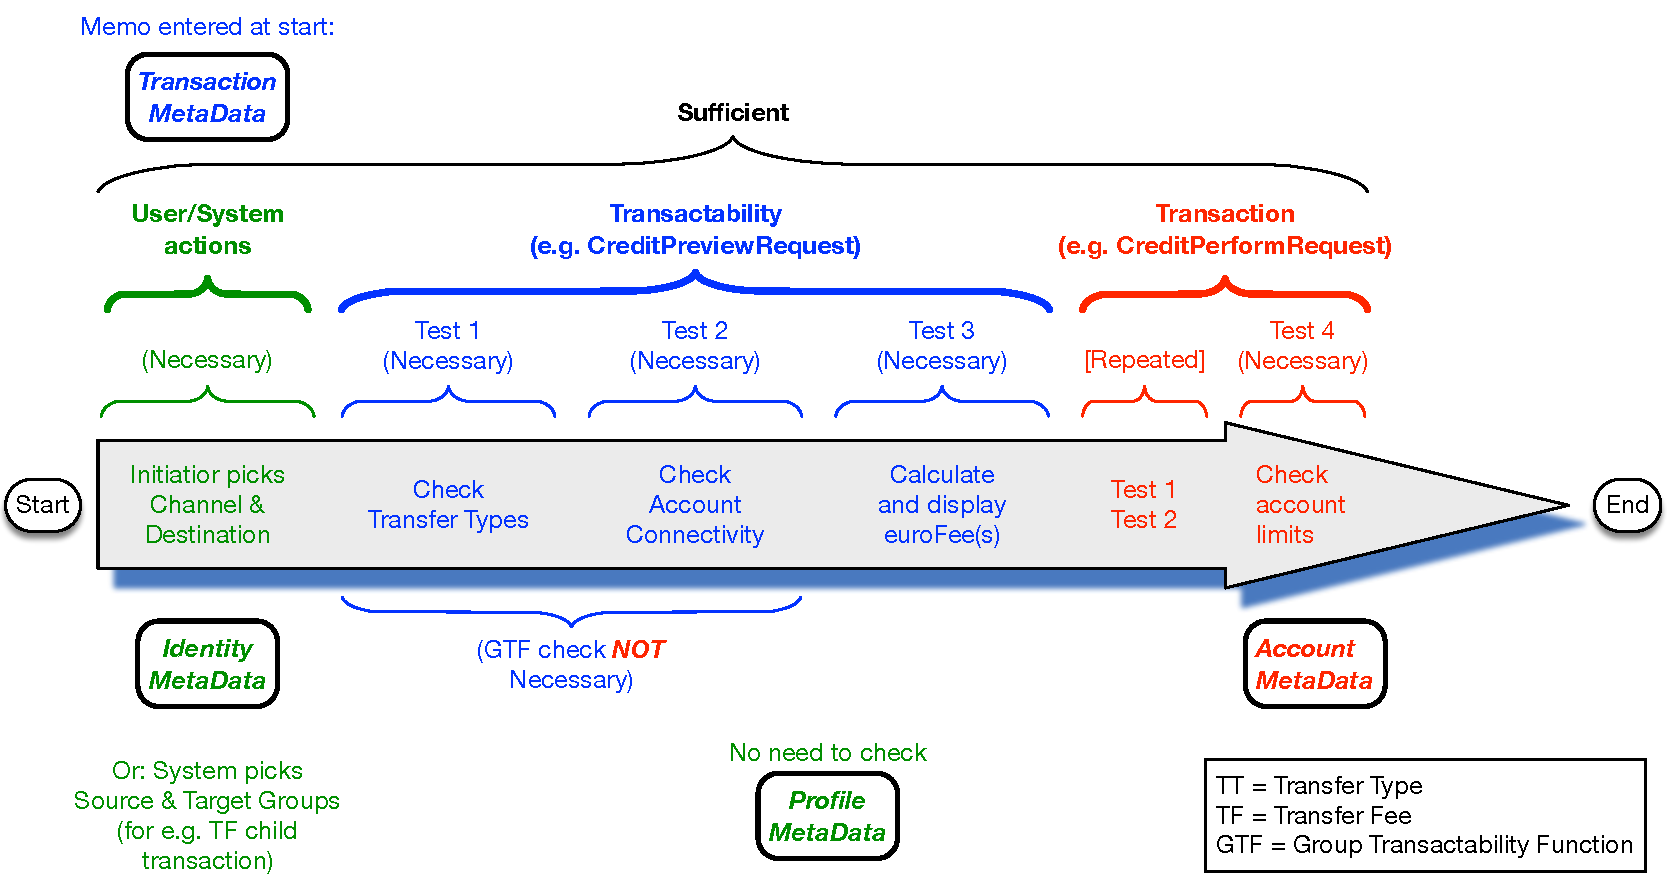
\includegraphics[width=16cm]{Figures/Transactability_Workflow}
\caption{\small\textbf{High-level workflow of the Permissioning process for user- or system-initiated transactions}}
\label{fig:transactabilitywkflow}
\end{figure}

\section{Detailed Discussion}

\subsection{Currencies and Channels}
As shown in Figure \ref{fig:currchan}, the Sardex/INTERLACE platform supports transactions in both Sardex credits (SRD) and Euros (Euro) over two kinds of channels. `Service' refers to transactions mediated either by a computer (web application) or a mobile phone (either a web application or a phone App). `POS' means `Point of Sale' and refers to the standard terminal used by retailers that accepts credit or debit cards, through which SRD transactions can be routed via an API. The figure also shows the four possible $\{ currency, channel \}$ combinations that we need to support in the definition and implementation of the permissioning tests discussed in the next sections.

\begin{figure}[htbp]
\centering
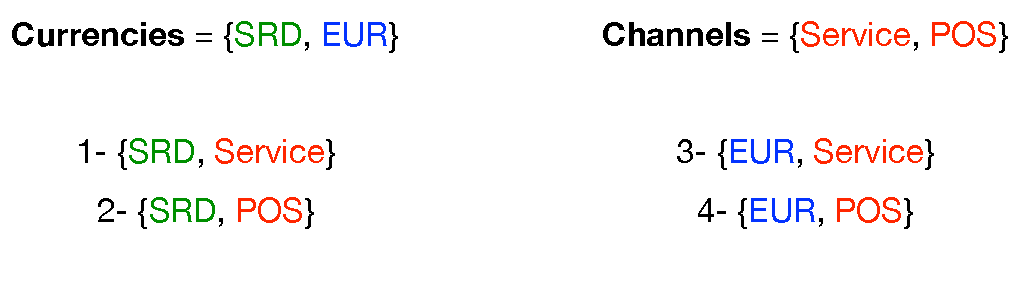
\includegraphics[width=10cm]{Figures/Curr_Chan}
\caption{\small\textbf{Currencies and channels supported by the platform}}
\label{fig:currchan}
\end{figure}

\subsection{Interaction Levels}
The interactions between circuit participants can be described from different points of view that correlate loosely to a stack view of the system. As shown in Figure \ref{fig:stack}, it is helpful to identify qualitatively the different levels of such a stack, acknowledging that it is \emph{more} than a networking communication stack in terms of scope but \emph{less} than one in terms of precision. `A' and `B' refer to the Initiator and the Target of the transaction, which do not necessarily correspond to the Buyer and the Seller.

\begin{figure}[htbp]
\centering
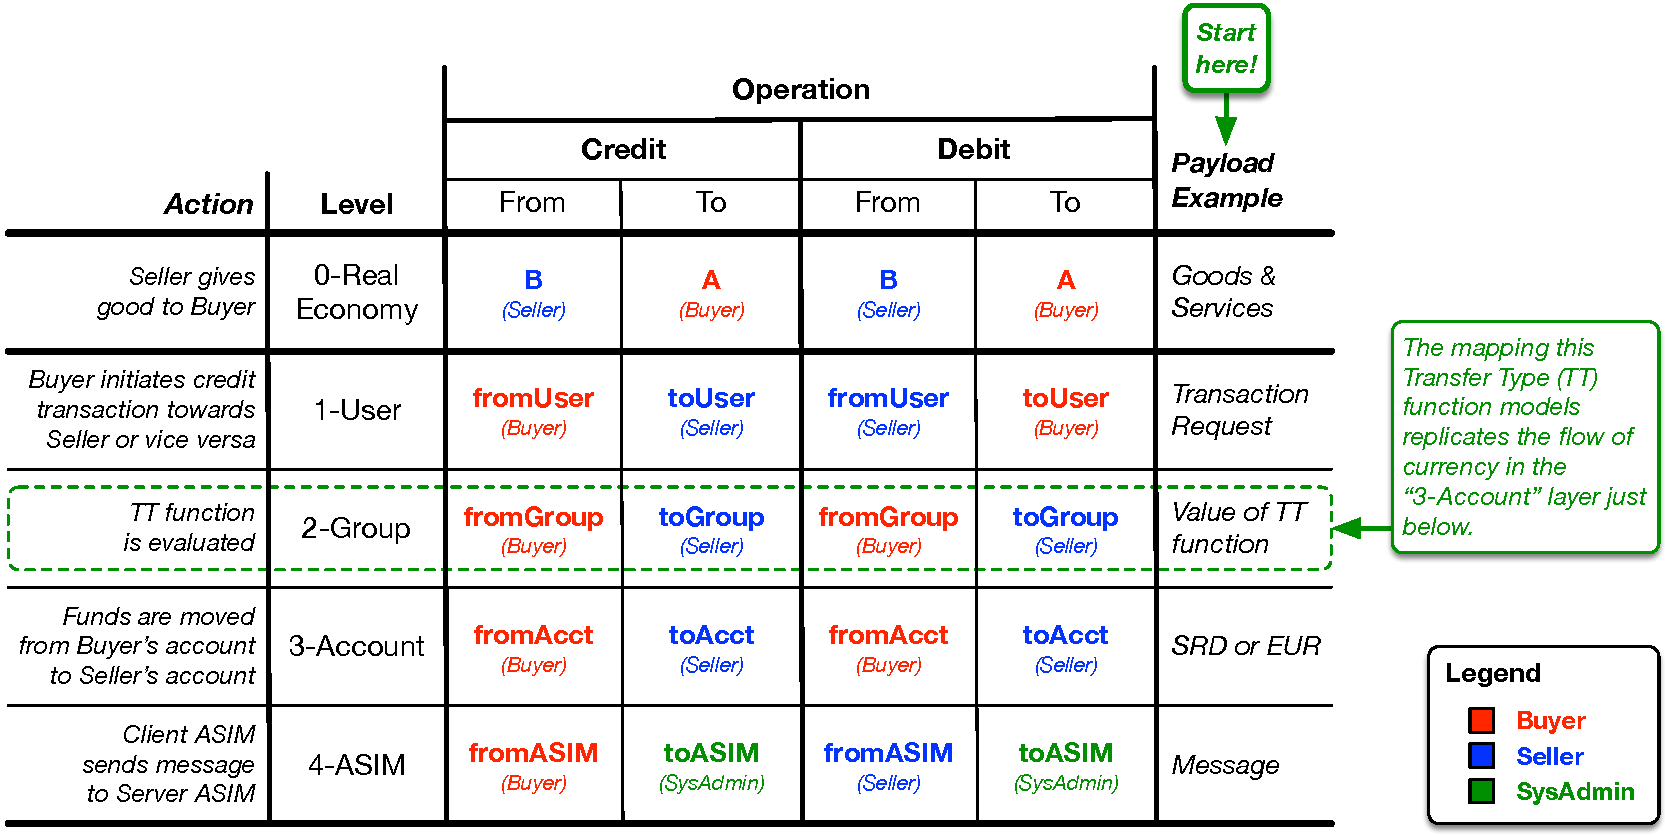
\includegraphics[width=10cm]{Figures/Stack}
\caption{\small\textbf{Stack view of the INTERLACE communication, economic, and financial  interactions}}
\label{fig:stack}
\end{figure}

Figure \ref{fig:stack} extends the two communication levels described in D2.1, but does so qualitatively. For the purposes of the implementation, we need a smaller set of levels but a more precise and specific vocabulary to identify the end-points of the transaction. Figure \ref{fig:vocabulary} shows this additional information as concerns levels 2, 3 and 4, which are labelled in the first column in the same way as in Figure \ref{fig:stack}, along with a great deal more information. In particular, this figure could be seen to integrate aspects of Figures \ref{fig:stack} and \ref{fig:transactabilitywkflow}, with the purpose of facilitating the conceptual understanding of the specification. `Groups' refer to user types, while `MetaData' to the parameters allocated to each user type or group. For example, the $\%$ of SRD accepted by a given user over 1000-EUR transaction values is a MetaData field of the Company group but not the Consumer\_Verified group.

\begin{figure}[htbp]
\centering
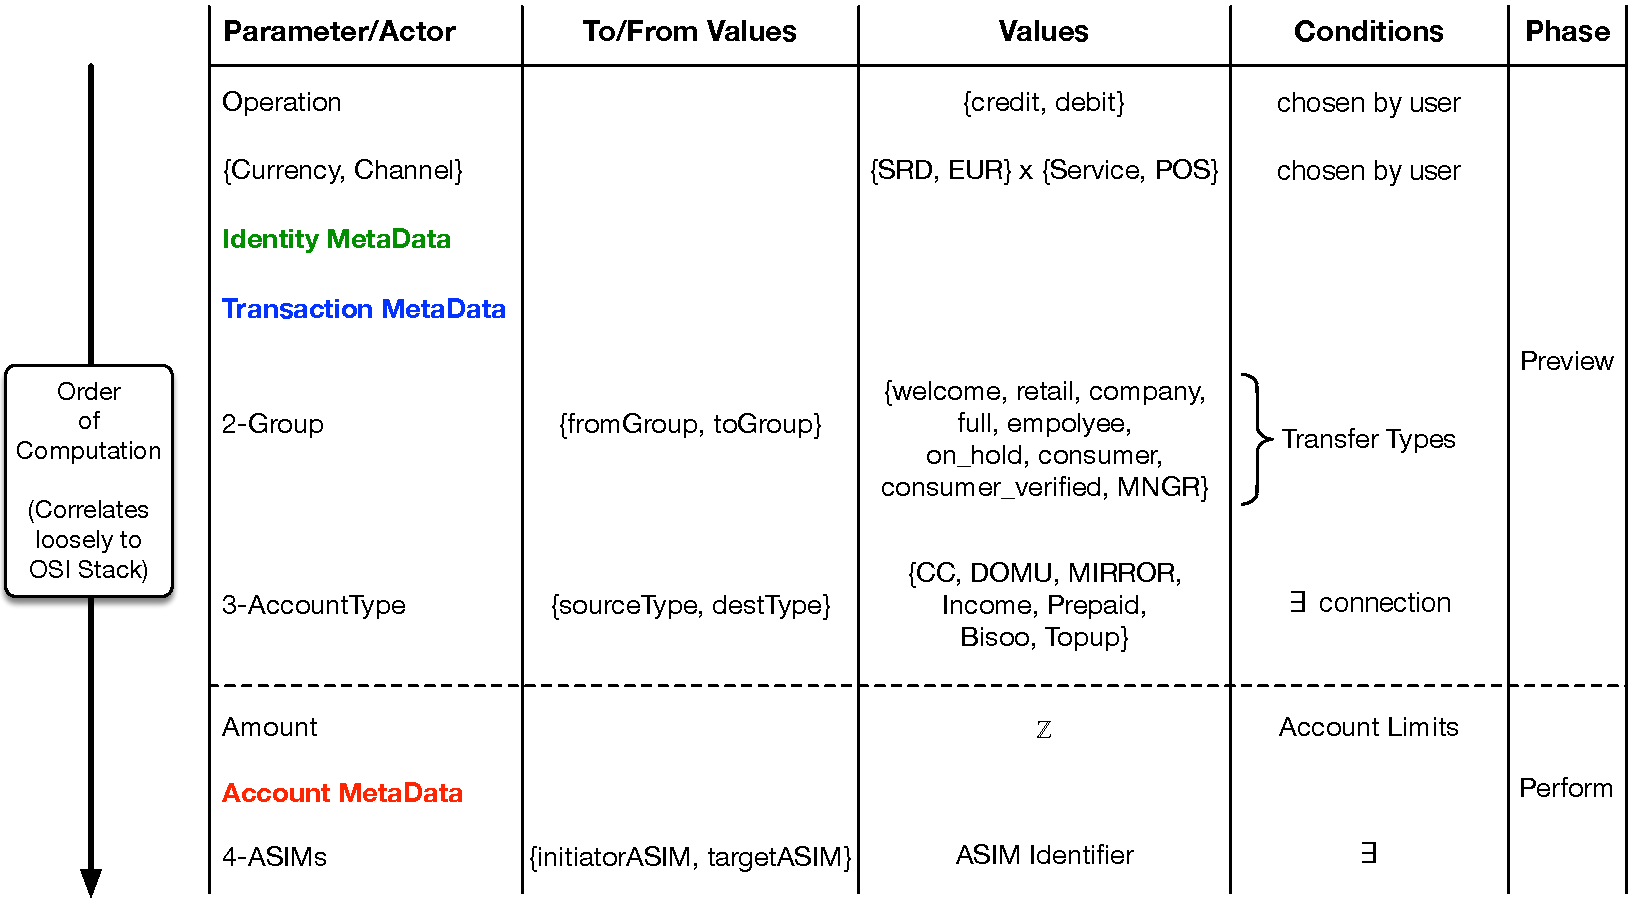
\includegraphics[width=17cm]{Figures/Vocabulary}
\caption{\small\textbf{Actors, parameters, levels, data structures, computational process, and conditions}}
\label{fig:vocabulary}
\end{figure}

\subsection{Visibility}
Before the initiator of a transaction can even issue a transaction request he/she must be able to \emph{see} the recipient. Figure \ref{fig:visibility}

\begin{figure}[htbp]
\centering
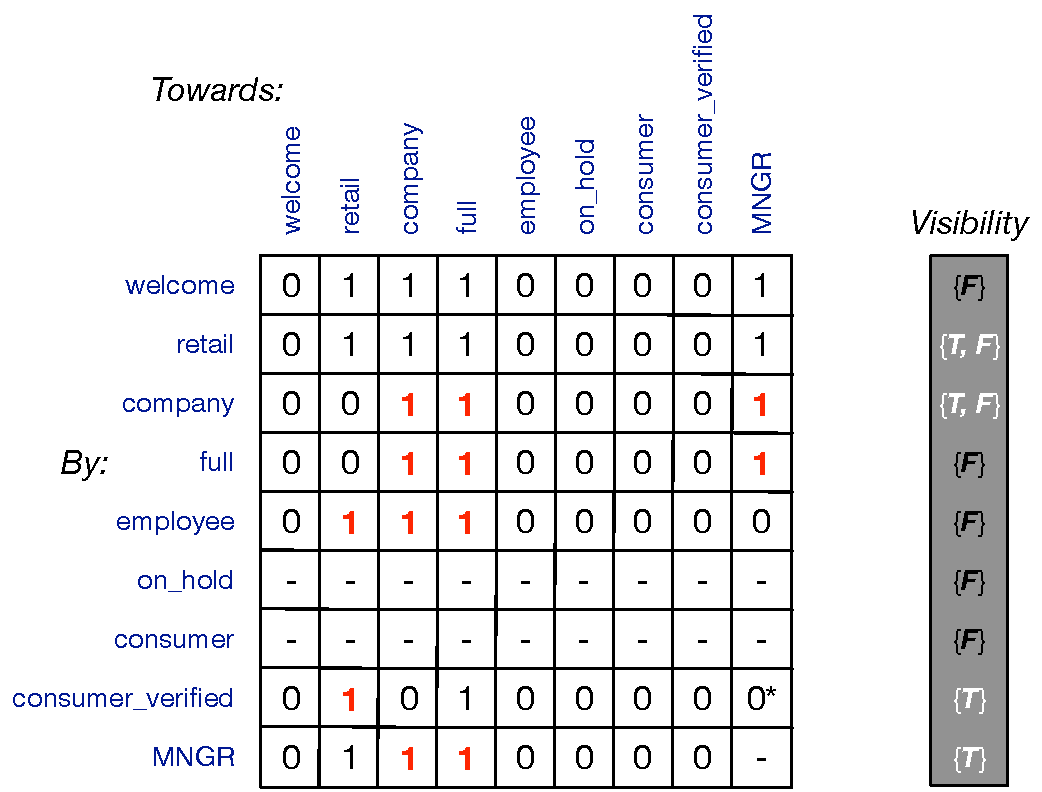
\includegraphics[width=10cm]{Figures/Visibility}
\caption{\small\textbf{Mutual visibility of different groups}}
\label{fig:visibility}
\end{figure}

























